{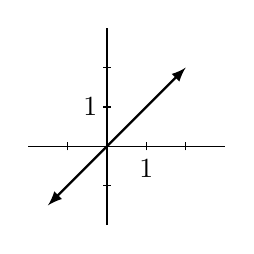
\begin{tikzpicture}[>=latex,scale=.5,baseline=10pt]
% Draw grid
\draw (-2,0)--(3,0);
\draw (0,-2)--(0,3);
\foreach \x in {-1,...,2}
 {\draw (\x,-.1)--(\x,.1);
 }
\foreach \y in {-1,...,2}
 {\draw (-.1,\y)--(.1,\y);
 };
\node[below] at (1,-0.1) {1};
\node[left] at (0,1) {1};

\draw[->,thick] (0,0) -- (2,2) node [right] {\vx};
\draw[->,thick] (0,0) -- (-1.5,-1.5) node [above left] {\vy};
\end{tikzpicture}}
{Sketches will vary depending on choice of origin of each vector.

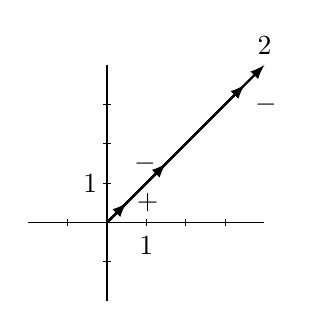
\begin{tikzpicture}[>=latex,scale=.5]
% Draw grid
\draw (-2,0)--(4,0);
\draw (0,-2)--(0,4);
\foreach \x in {-1,...,3}
 {\draw (\x,-.1)--(\x,.1);
 }
\foreach \y in {-1,...,3}
 {\draw (-.1,\y)--(.1,\y);
 };
\node[below] at (1,-0.1) {1};
\node[left] at (0,1) {1};

\draw[->,thick] (0,0) -- (4,4) node [above] {$2\vx$};
\draw[->,thick] (0,0) -- (1.5,1.5) node [left] {$-\vy$};
\draw[->,thick] (0,0) -- (.5,.5) node [right] {$\vx+\vy$};
\draw[->,thick] (0,0) -- (3.5,3.5) node [below right] {$\vx-\vy$};

\end{tikzpicture}
}